\documentclass{article}
\usepackage[x11names, rgb]{xcolor}
\usepackage[utf8]{inputenc}
\usepackage{tikz}
\usetikzlibrary{snakes,arrows,shapes}
\usepackage{amsmath}

\usetikzlibrary{automata}%

\begin{document}
\pagestyle{empty}
\ \\
notacija: $ input,\ pop \rightarrow push$ \\ 
torej ko imamo vhodni znak $input$ vzamemo iz sklada $pop$ in damo na sklad $push$ \\
\ \\
\enlargethispage{100cm}
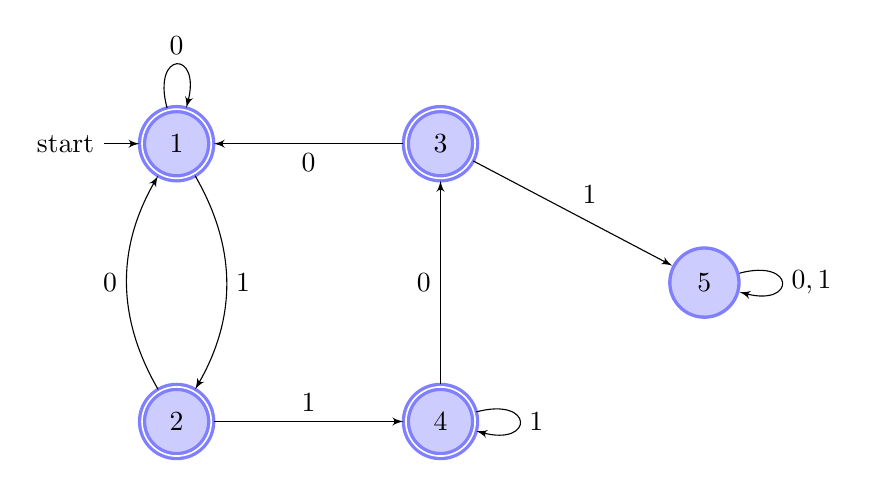
\begin{tikzpicture}[>=latex',join=bevel,]
\tikzstyle{every state}=     [draw=blue!50,very thick,fill=blue!20]%
  \node (1) at (0bp,105bp) [state,initial, accepting] {1};
  \node (2) at (0bp,05bp) [state,accepting] {2};
  \node (3) at (95bp,105bp) [state,accepting] {3};
  \node (4) at (95bp,05bp) [state,accepting] {4};
  \node (5) at (190bp,55bp) [state] {5};
  
  \draw [->] (1) to[loop above] node[auto] { $ 0 $ } (1);
  \draw [->] (1) to[bend left] node[auto] { $ 1 $ } (2);
  \draw [->] (2) to[bend left] node[auto] { $ 0 $ } (1);
  \draw [->] (2) to[right] node[auto] { $ 1 $ } (4);
  \draw [->] (4) to[loop right] node[auto] { $ 1 $ } (4);
  \draw [->] (4) to[right] node[auto] { $ 0 $ } (3);
  \draw [->] (3) to[right] node[auto] { $ 0 $ } (1);
  \draw [->] (3) to[right] node[auto] { $ 1 $ } (5);
  \draw [->] (5) to[loop right] node[auto] { $ 0,1 $ } (5);


\end{tikzpicture}
\\
\\
\end{document}


